

\tikzset{every picture/.style={line width=0.75pt}} %set default line width to 0.75pt        

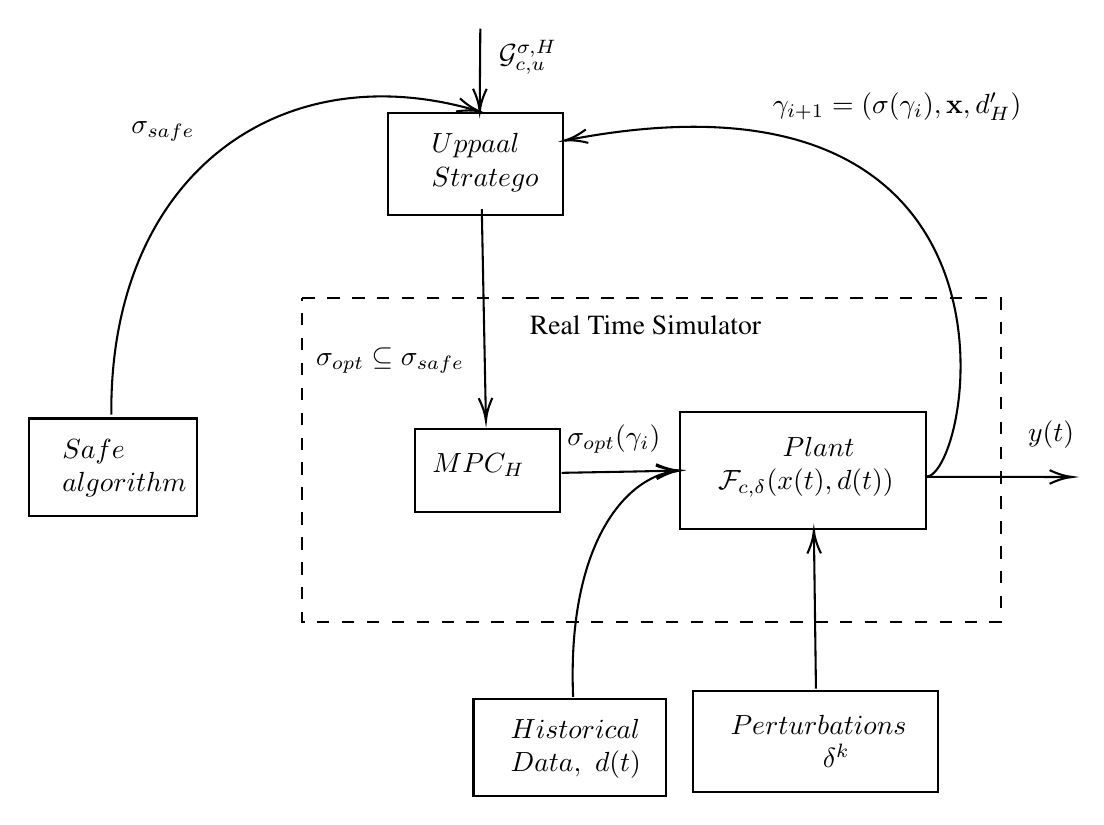
\begin{tikzpicture}[x=0.75pt,y=0.75pt,yscale=-1,xscale=1]
%uncomment if require: \path (0,419); %set diagram left start at 0, and has height of 419

%Shape: Rectangle [id:dp7947774674470398] 
\draw  [dash pattern={on 4.5pt off 4.5pt}] (232.8,147) -- (569.29,147) -- (569.29,303.11) -- (232.8,303.11) -- cycle ;
%Shape: Rectangle [id:dp581005149361487] 
\draw   (274,58) -- (358.29,58) -- (358.29,107.11) -- (274,107.11) -- cycle ;

%Shape: Rectangle [id:dp014468904493361467] 
\draw   (101,205) -- (182.29,205) -- (182.29,252.11) -- (101,252.11) -- cycle ;

%Curve Lines [id:da5102886223745438] 
\draw    (533.29,233.11) .. controls (555.29,233.11) and (593.29,25.11) .. (359.29,71.11) ;
\draw [shift={(359.29,71.11)}, rotate = 348.88] [color={rgb, 255:red, 0; green, 0; blue, 0 }  ][line width=0.75]    (10.93,-3.29) .. controls (6.95,-1.4) and (3.31,-0.3) .. (0,0) .. controls (3.31,0.3) and (6.95,1.4) .. (10.93,3.29)   ;
%Curve Lines [id:da5736171914204411] 
\draw    (140.8,203.2) .. controls (139.8,87.78) and (221.97,28.79) .. (316.86,56.68) ;
\draw [shift={(318.29,57.11)}, rotate = 196.84] [color={rgb, 255:red, 0; green, 0; blue, 0 }  ][line width=0.75]    (10.93,-3.29) .. controls (6.95,-1.4) and (3.31,-0.3) .. (0,0) .. controls (3.31,0.3) and (6.95,1.4) .. (10.93,3.29)   ;
%Straight Lines [id:da7885671872764144] 
\draw    (318.58,17.22) -- (318.3,55.11) ;
\draw [shift={(318.29,57.11)}, rotate = 270.42] [color={rgb, 255:red, 0; green, 0; blue, 0 }  ][line width=0.75]    (10.93,-3.29) .. controls (6.95,-1.4) and (3.31,-0.3) .. (0,0) .. controls (3.31,0.3) and (6.95,1.4) .. (10.93,3.29)   ;
%Shape: Rectangle [id:dp946630032262731] 
\draw   (315.29,340.11) -- (408,340.11) -- (408,387) -- (315.29,387) -- cycle ;

%Shape: Rectangle [id:dp718981269708326] 
\draw   (421,336.11) -- (539.29,336.11) -- (539.29,385.11) -- (421,385.11) -- cycle ;

%Shape: Rectangle [id:dp45733661710220663] 
\draw   (415,202) -- (533.29,202) -- (533.29,258.11) -- (415,258.11) -- cycle ;

%Straight Lines [id:da8932062177607605] 
\draw    (319.29,104.11) -- (321.25,204.11) ;
\draw [shift={(321.29,206.11)}, rotate = 268.88] [color={rgb, 255:red, 0; green, 0; blue, 0 }  ][line width=0.75]    (10.93,-3.29) .. controls (6.95,-1.4) and (3.31,-0.3) .. (0,0) .. controls (3.31,0.3) and (6.95,1.4) .. (10.93,3.29)   ;
%Straight Lines [id:da8287101777047321] 
\draw    (480.29,335.11) -- (479.32,261.11) ;
\draw [shift={(479.29,259.11)}, rotate = 449.25] [color={rgb, 255:red, 0; green, 0; blue, 0 }  ][line width=0.75]    (10.93,-3.29) .. controls (6.95,-1.4) and (3.31,-0.3) .. (0,0) .. controls (3.31,0.3) and (6.95,1.4) .. (10.93,3.29)   ;
%Shape: Rectangle [id:dp34848466006382406] 
\draw   (287,210) -- (357,210) -- (357,250) -- (287,250) -- cycle ;
%Curve Lines [id:da1228487673215457] 
\draw    (363.29,339.11) .. controls (360.36,267.93) and (386.91,233.83) .. (412.34,230.32) ;
\draw [shift={(414.29,230.11)}, rotate = 535.6] [color={rgb, 255:red, 0; green, 0; blue, 0 }  ][line width=0.75]    (10.93,-3.29) .. controls (6.95,-1.4) and (3.31,-0.3) .. (0,0) .. controls (3.31,0.3) and (6.95,1.4) .. (10.93,3.29)   ;
%Straight Lines [id:da8899650593931607] 
\draw    (357.8,231.2) -- (392.81,230.56) -- (412.29,230.15) ;
\draw [shift={(414.29,230.11)}, rotate = 538.79] [color={rgb, 255:red, 0; green, 0; blue, 0 }  ][line width=0.75]    (10.93,-3.29) .. controls (6.95,-1.4) and (3.31,-0.3) .. (0,0) .. controls (3.31,0.3) and (6.95,1.4) .. (10.93,3.29)   ;
%Straight Lines [id:da6729134920451438] 
\draw    (533.29,233.11) -- (601.8,233.2) ;
\draw [shift={(603.8,233.2)}, rotate = 180.07] [color={rgb, 255:red, 0; green, 0; blue, 0 }  ][line width=0.75]    (10.93,-3.29) .. controls (6.95,-1.4) and (3.31,-0.3) .. (0,0) .. controls (3.31,0.3) and (6.95,1.4) .. (10.93,3.29)   ;

% Text Node
\draw (287,64.4) node [anchor=north west][inner sep=0.75pt]    {$ \begin{array}{l}
Uppaal\\
Stratego
\end{array}$};
% Text Node
\draw (109,211.51) node [anchor=north west][inner sep=0.75pt]    {$ \begin{array}{l}
Safe\ \\
algorithm
\end{array}$};
% Text Node
\draw (149,60.4) node [anchor=north west][inner sep=0.75pt]    {$\sigma _{safe}$};
% Text Node
\draw (458,46.4) node [anchor=north west][inner sep=0.75pt]    {$\gamma _{i+1} =( \sigma ( \gamma _{i}) ,\mathbf{x} ,d'_{H})$};
% Text Node
\draw (238,169.4) node [anchor=north west][inner sep=0.75pt]    {$\sigma _{opt} \subseteq \sigma _{safe}$};
% Text Node
\draw (326,21.4) node [anchor=north west][inner sep=0.75pt]    {$\mathcal{G}_{c,u}^{\sigma ,H}$};
% Text Node
\draw (325,346.4) node [anchor=north west][inner sep=0.75pt]    {$ \begin{array}{l}
Historical\ \\
Data,\ d( t)
\end{array}$};
% Text Node
\draw (431,344.4) node [anchor=north west][inner sep=0.75pt]    {$ \begin{array}{l}
Perturbations\\
\ \ \ \ \ \ \ \ \ \ \delta ^{k}
\end{array}$};
% Text Node
\draw (425,210.4) node [anchor=north west][inner sep=0.75pt]    {$ \begin{array}{l}
\ \ \ \ \ \ \ Plant\ \\
\mathcal{F}_{c,\delta }( x( t) ,d( t))
\end{array}$};
% Text Node
\draw (294,220.4) node [anchor=north west][inner sep=0.75pt]    {$MPC_{H}$};
% Text Node
\draw (341,154) node [anchor=north west][inner sep=0.75pt]   [align=left] {{\fontfamily{ptm}\selectfont Real Time Simulator}};
% Text Node
\draw (359,206.4) node [anchor=north west][inner sep=0.75pt]    {$\sigma _{opt}( \gamma _{i})$};
% Text Node
\draw (581,204.4) node [anchor=north west][inner sep=0.75pt]    {$y( t)$};


\end{tikzpicture}
